\documentclass[conference]{IEEEtran}
\IEEEoverridecommandlockouts
% The preceding line is only needed to identify funding in the first footnote. If that is unneeded, please comment it out.
\usepackage{cite}
\usepackage{amsmath,amssymb,amsfonts}
\usepackage{algorithmic}
\usepackage{algorithm}
\usepackage{graphicx}
\usepackage{textcomp}
\usepackage{float}
\usepackage{xcolor}
\usepackage{amssymb}

\newtheorem{theorem}{Theorem}
\newtheorem{proof}{Proof}
\def\BibTeX{{\rm B\kern-.05em{\sc i\kern-.025em b}\kern-.08em
    T\kern-.1667em\lower.7ex\hbox{E}\kern-.125emX}}
\begin{document}

\title{TLBO-HHO AoI-Aware Task Offloading for Mobile Edge Computing
\thanks{This work is supported by the Beijing Natural Science Foundation (No. L222048 and No. L233005)}
\thanks{* Corresponding author: Haoru Su (email: suhaoru@bjut.edu.cn).}
}

\author{\IEEEauthorblockN{1\textsuperscript{st} Jie Bai}
\IEEEauthorblockA{\textit{College of Computer Science} \\
\textit{Beijing University of Technology}\\
Beijing, China \\
baijie0219@gmail.com}
\and
\IEEEauthorblockN{2\textsuperscript{nd} Haoru Su\textsuperscript{*}}
\IEEEauthorblockA{\textit{College of Computer Science} \\
\textit{Beijing University of Technology}\\
Beijing, China \\
suhaoru@bjut.edu.cn}
\and
\IEEEauthorblockN{3\textsuperscript{rd} Jing Bi}
\IEEEauthorblockA{\textit{College of Computer Science} \\
\textit{Beijing University of Technology}\\
Beijing, China \\
bijing@bjut.edu.cn}
\and
\IEEEauthorblockN{4\textsuperscript{th} Li Zhang}
\IEEEauthorblockA{\textit{College of Computer Science} \\
\textit{Beijing University of Technology}\\
Beijing, China \\
zhangli828@bjut.edu.cn}
\and
\IEEEauthorblockN{5\textsuperscript{th} Xiaoming Yuan}
\IEEEauthorblockA{\textit{Qinhuangdao Branch Campus} \\
\textit{Northeastern University}\\
Qinhuangdao, China \\
yuanxiaoming@neuq.edu.cn}
\and
\IEEEauthorblockN{6\textsuperscript{th} Xiliang Liu}
\IEEEauthorblockA{\textit{College of Computer Science} \\
\textit{Beijing University of Technology}\\
Beijing, China \\
liuxl@bjut.edu.cn}
}

\maketitle

\begin{abstract}
\textbf{Mobile Edge Computing (MEC) emerges as a paradigm shift in distributed computing, bringing computational resources closer to end-users to support latency-sensitive and computation-intensive applications in 5G/6G networks. However, task offloading in MEC environments faces critical challenges: the inherent trade-offs between energy consumption and processing latency, the dynamic nature of wireless channels affecting transmission reliability, and the increasing demand for real-time information freshness in IoT applications. This work proposes a two-phase integrated Teaching-Learning-Based Optimization and Harris Hawks Optimization (TLBO-HHO) algorithm to address this tri-objective optimization problem. We establish an optimization model incorporating Age of Information (AoI) as a key metric for information freshness, prove its NP-hardness, and develop an adaptive switching mechanism that balances global exploration and local exploitation. Experimental results demonstrate that TLBO-HHO achieves fitness value improvements of 54.5\%, 63.5\%, and 76.2\% compared to three other existing mechanisms, while maintaining an average AoI of 1.68s through intelligent resource allocation strategies.}
\end{abstract}

\begin{IEEEkeywords}
mobile edge computing, task offloading, age of information, TLBO-HHO algorithm
\end{IEEEkeywords}

\section{Introduction}
\IEEEPARstart{W}{ith} the rapid development of Internet of Things (IoT) and 5G/6G communication technologies, the amount of data generated by mobile devices is growing exponentially. Mobile Edge Computing (MEC) provides an effective solution for delay-sensitive applications by deploying computing resources at the network edge~\cite{mao2017survey}. In MEC systems, task offloading represents a fundamental decision-making process where mobile devices determine whether to execute computational tasks locally or delegate them to edge servers. 

This decision faces significant challenges in balancing multiple conflicting objectives. First, the energy consumption of resource-constrained mobile devices must be minimized to extend battery life, while processing latency needs to be reduced to meet real-time application requirements. Second, the heterogeneity of devices and tasks complicates resource allocation decisions. Third, maintaining information freshness for time-sensitive applications adds another dimension to the optimization problem. Traditional approaches have primarily focused on energy-latency trade-offs using mathematical optimization~\cite{wang2017joint} or machine learning techniques~\cite{wang2021deep}. However, these methods often struggle with scalability in non-convex problem spaces or require extensive training data. Moreover, existing solutions rarely consider information freshness, leading to suboptimal performance in real-time monitoring and control applications where outdated information can severely impact system functionality.

In addition, Age of Information (AoI) has emerged as a critical metric for quantifying the timeliness of information at the receiver. First introduced by Kaul \textit{et al.}~\cite{kaul2012real}, AoI measures the time elapsed since the generation of the most recently received update, becoming particularly important in status update systems and real-time monitoring applications. Motivated also by recent hybrid metaheuristic advances — e.g., hybrid FPA–TS for edge–cloud resource allocation in IoT environments~\cite{Dankolo_2025}, and quantum‑inspired hybrid evolutionary algorithms for QoS enhancement in IoT service management~\cite{Singh_2025} — the integration of AoI into MEC task offloading presents new challenges, as traditional approaches focusing solely on energy and latency may fail to ensure timely information delivery.

This paper proposes a novel two-phase integrated algorithm combining Teaching-Learning-Based Optimization (TLBO) and Harris Hawks Optimization (HHO) to address the multi-objective task offloading problem in MEC environments. We establish a comprehensive optimization model that jointly considers energy consumption, processing latency, and AoI, proving its NP-hard nature through reduction to the knapsack problem. The proposed TLBO-HHO algorithm employs an adaptive switching mechanism that leverages TLBO's stable convergence properties for local exploitation and HHO's dynamic search capabilities for global exploration. Through extensive experimental evaluation, our approach demonstrates significant performance improvements: achieving superior fitness values with percentage improvements of 65.2\%, 85.4\%, and 74.6\% compared to standalone TLBO, GA, and GWO algorithms respectively. Moreover, the algorithm successfully maintains information freshness with 95\% of real-time sensitive tasks achieving AoI below 1 second, while reducing average energy consumption by 40.3\% compared to baseline approaches.

\section{Related work}

The task offloading optimization problem in MEC has been extensively studied through various methodological approaches. In the domain of metaheuristic algorithms, TLBO and HHO show promising results for complex optimization problems. In~\cite{rao2011teaching}, TLBO is proposed to simulate the classroom teaching process, demonstrating parameter-free operation and stable convergence characteristics. In~\cite{heidari2019harris}, HHO is introduced to mimic the cooperative hunting behavior of Harris hawks, showing effectiveness in handling multimodal optimization landscapes. Recent studies explore hybridization strategies; in~\cite{chen2020multi}, Chen \textit{et al.} develop a multi-population differential evolution-assisted HHO framework, while in~\cite{tu2023hybrid}, Tu \textit{et al.} propose a hybrid algorithm combining grey wolf optimizer with HHO for global optimization problems.

For MEC task offloading specifically, existing optimization methods fall into three main categories. Mathematical optimization methods provide theoretical foundations but face limitations in practical scenarios. In~\cite{wang2017joint}, a joint computation offloading and interference management scheme based on Lagrangian dual decomposition is developed, offering optimal solutions under convex assumptions. In~\cite{liu2016delay}, a Lyapunov optimization-based algorithm is proposed for delay-optimal task scheduling, ensuring queue stability while minimizing average delay. However, these methods struggle with the non-convex nature of real-world MEC systems and often require simplifying assumptions that limit their applicability.

Machine learning approaches gain traction for their adaptability to dynamic environments. In~\cite{wang2021deep}, a deep reinforcement learning-based dynamic trajectory control scheme is presented for UAV-assisted MEC, demonstrating adaptive resource allocation capabilities. In~\cite{zang2022federated}, federated deep reinforcement learning is integrated into the optimization framework, addressing privacy concerns while optimizing task offloading decisions. Despite their advantages, these methods require extensive training data and computational resources, making them less suitable for resource-constrained scenarios.

Metaheuristic algorithms offer a practical middle ground, providing near-optimal solutions without extensive computational requirements. In~\cite{li2020genetic}, genetic algorithms are applied to MEC task offloading, achieving energy consumption reduction through evolutionary optimization. In~\cite{ali2024multiobjective}, a multi-objective HHO algorithm is developed for task scheduling in cloud-fog computing, demonstrating effectiveness in handling NP-hard problems. These approaches show promise but often focus on traditional objectives without considering information freshness.

Recent research begins incorporating AoI into MEC optimization frameworks. In~\cite{liu2023asynchronous}, an asynchronous deep reinforcement learning method is proposed for AoI-aware task computing in vehicular edge computing, jointly optimizing computing resource allocation and information freshness. In~\cite{zhou2019computation}, a contract matching mechanism considering AoI is designed for vehicular fog computing, achieving efficient resource allocation while maintaining timely updates. However, existing work primarily relies on learning-based or game-theoretic approaches, with limited exploration of metaheuristic algorithms for AoI-aware optimization.

Furthermore, hybrid metaheuristic frameworks recently emerge: Zheng \textit{et al.}~\cite{Zheng_2025} propose a hybrid metaheuristic-based UAV trajectory and offloading optimization strategy, demonstrating improved performance in MEC settings, while Perera \textit{et al.}~\cite{Perera_2025} combine reinforcement learning with adaptive PSO for IIoT task offloading, achieving significant gains in dynamic environments. These studies align with our theme of hybrid approaches but differ by emphasizing UAV mobility or RL-PSO control.

Current approaches exhibit several limitations: mathematical optimization methods struggle with non-convexity and scalability; machine learning approaches require extensive training and may not generalize well; existing metaheuristic algorithms often consider only traditional objectives without AoI awareness; and the potential of hybrid metaheuristic algorithms for comprehensive multi-objective optimization remains underexplored. These observations motivate our work on developing a hybrid TLBO-HHO algorithm that addresses energy, latency, and AoI objectives simultaneously while maintaining computational efficiency and solution quality.

\section{System Model and Problem Statement}

We consider a three-layer MEC network architecture comprising mobile devices, edge servers, and cloud servers, as illustrated in Fig.~\ref{fig1}. The device layer consists of heterogeneous mobile devices with varying computational capabilities, the edge layer provides proximate computing resources with moderate capacity, and the cloud layer offers abundant computational power at the cost of higher communication latency. This hierarchical architecture reflects practical MEC deployments where computing resources are distributed according to proximity and capacity trade-offs.

\begin{figure}[!t]
    \centering
    \centerline{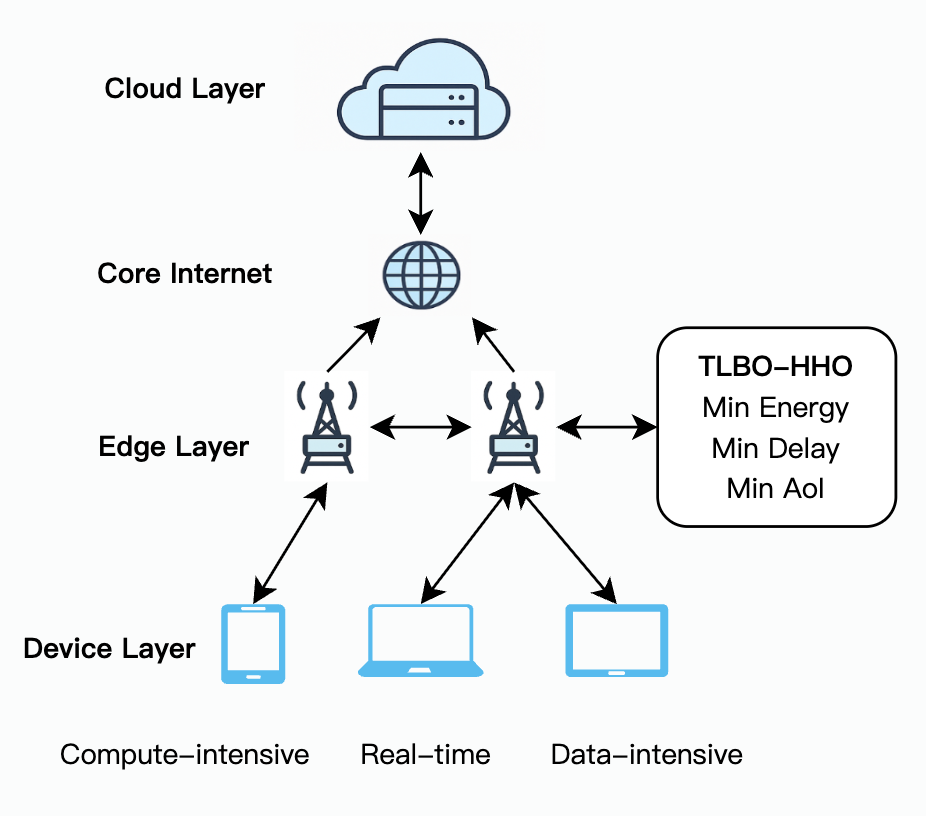
\includegraphics[width=1.0\linewidth]{mec_image1.png}}
    \caption{Device-Edge-Cloud network architecture.}
    \label{fig1}
\end{figure}

\subsection{\textit{Computation Model}}
\subsubsection{Task Characteristics}
Each task $i \in \mathcal{T}$ is characterized by a five-tuple:
\begin{equation}
\tau_i = (D_i, C_i, T_i^{\max}, \lambda_i, AoI_i^{\max})
\end{equation}
where:
\begin{itemize}
    \item $D_i$ is the input data size (MB), $D_i^{result}$ is the output data size
    \item $C_i$ is the computational complexity (CPU cycles/bit)
    \item $T_i^{\max}$ is the maximum tolerable delay (s)
    \item $\lambda_i$ is the task update interval (s)
    \item $AoI_i^{\max}$ is the maximum acceptable age of information (s)
\end{itemize}

\subsubsection{Delay Model}
The total task processing delay includes transmission delay, waiting delay, and computation delay:
\begin{equation}
T_i = T_i^{trans} + T_i^{wait} + T_i^{comp}
\end{equation}

Local execution delay only includes computation time:
\begin{equation}
T_{i,d(i)}^{local} = \frac{D_i \cdot C_i}{f_{i,d(i)}}
\end{equation}
where $f_{i,d(i)}$ is the CPU frequency allocated to task $i$.

The delay for offloading a task to an edge server:
\begin{equation}
T_{i,d(i),e(i)}^{edge} = \frac{D_i}{R_{d(i),e(i)}} + T_{queue}^{edge} + \frac{D_i \cdot C_i}{f_{i,e(i)}} + \frac{D_i^{result}}{R_{e(i),d(i)}}
\end{equation}
where $R_{j,k}$ is the transmission rate from node $j$ to $k$, calculated using Shannon's formula:
\begin{equation}
R_{j,k} = B_{j,k} \log_2\left(1 + \frac{P_j^{trans} \cdot h_{j,k}}{N_0 \cdot B_{j,k}}\right)
\end{equation}

\textbf{Queuing delay analysis}: Considering edge servers adopt the M/M/1 queuing model, the average waiting time is:
\begin{equation}
T_{queue}^{edge} = \frac{\rho}{f_e \cdot (1-\rho)}
\end{equation}
where $\rho = \lambda_e / \mu_e$ is the server utilization rate, $\lambda_e$ is the task arrival rate, and $\mu_e$ is the service rate.

\subsubsection{Energy Model}
Computation energy consumption adopts a dynamic power model:
\begin{equation}
E_{i,j}^{comp} = \kappa_j \cdot (f_{i,j})^{\alpha} \cdot D_i \cdot C_i
\end{equation}
where $\kappa_j \in [1.0, 3.5] \times 10^{-27}$ and $\alpha \in [2.2, 2.8]$ are set according to device type.

Transmission energy consumption: $E_{i,j,k}^{trans} = P_j^{trans} \cdot (D_i + D_i^{result})/R_{j,k}$, where $P_j^{trans} \in [0.1, 0.5]$ W.

The total energy consumption of mobile devices:
\begin{equation}
    \begin{split}
        E_i = x_{i}^{local} \cdot E_{i,d(i)}^{comp} + x_{i}^{edge} \cdot E_{i,d(i),e(i)}^{trans} \\ + x_{i}^{cloud} \cdot (E_{i,d(i),e(i)}^{trans} + E_{i,e(i),c(i)}^{trans})
    \end{split}
\end{equation}

\subsubsection{AoI Model}
To describe the freshness of information, we define the Age of Information (AoI) metric. For task $i$, its AoI at time $t$ is defined as:
\begin{equation}
AoI_i(t) = t - U_i(t)
\end{equation}
where $U_i(t)$ is the time when task $i$ last successfully completed an update.

Considering task processing delay and update interval, the average AoI of task $i$ is:
\begin{equation}
\overline{AoI}_i = \lambda_i + \frac{T_i}{2} + \frac{T_i^2}{2\lambda_i}
\end{equation}

This formula considers three parts: update interval $\lambda_i$, average waiting time $T_i/2$, and additional aging due to processing delay $T_i^2/(2\lambda_i)$.

\subsection{\textit{Optimization Problem Modeling}}
\subsubsection{Decision Variables}
We define binary decision variables $\mathbf{x} = \{x_i^{local}, x_i^{edge}, x_i^{cloud}\}_{i \in \mathcal{T}}$, where:
\begin{itemize}
    \item $x_{i}^{local}$ indicates task $i$ is executed locally on the device
    \item $x_{i}^{edge}$ indicates task $i$ is offloaded to an edge server
    \item $x_{i}^{cloud}$ indicates task $i$ is offloaded to a cloud server
\end{itemize}
Continuous decision variables $\mathbf{f} = \{f_{i,j}\}_{i \in \mathcal{T}, j \in \mathcal{D} \cup \mathcal{E} \cup \mathcal{C}}$ represent the allocated CPU frequency.

\subsubsection{Objective Function}
Based on practical application requirements and recent research trends, we use the weighted sum method to transform the tri-objective into a single objective:
\begin{equation}
    \begin{split}
        \min_{\mathbf{x}, \mathbf{f}} F = \sum_{i \in \mathcal{T}} \bigg( w^E \cdot \frac{E_i}{E^{norm}} + w^T \cdot \frac{T_i}{T^{norm}}
        \\+ w^{AoI} \cdot \frac{\overline{AoI}_i}{AoI^{norm}} \bigg)
    \end{split}
\end{equation}
where:
\begin{itemize}
    \item Weight settings: $w^E = 0.25$, $w^T = 0.35$, $w^{AoI} = 0.40$ (prioritizing information timeliness)
    \item Normalization factors: $E^{norm} = \max_{i \in \mathcal{T}} E_i^{local}$, $T^{norm} = \max_{i \in \mathcal{T}} T_i^{cloud}$, $AoI^{norm} = \max_{i \in \mathcal{T}} AoI_i^{\max}$
\end{itemize}

\subsubsection{Constraints}
The optimization is subject to the following constraints:
\begin{itemize}
    \item[a.] Task allocation uniqueness: $x_{i}^{local} + x_{i}^{edge} + x_{i}^{cloud} = 1, \forall i$
    \item[b.] Resource capacity: $\sum_{i} x_{i}^{j} \cdot f_{i,j} \leq F_{j}^{\max}, \forall j$
    \item[c.] Delay constraint: $T_i \leq T_i^{\max}, \forall i$
    \item[d.] AoI constraint: $\overline{AoI}_i \leq AoI_i^{\max}, \forall i$
    \item[e.] Quality of service: At least 95\% of tasks meet delay requirements
\end{itemize}

\subsubsection{Problem Complexity Analysis}

\textbf{Theorem 1}: The MEC task offloading and resource allocation problem considering AoI is NP-hard.

\textit{Proof}: Consider a special instance: only one edge server ($E = 1$), all tasks have the same data size $D$ and computational complexity $C$, and transmission delay and AoI constraints are ignored. In this case, the problem is equivalent to:
\begin{equation}
    \begin{split}
        \min_{S \subseteq \mathcal{T}} \sum_{i \in S} p_i, \quad
        \text{s.t.} \quad p_i = \frac{DC}{f_i}, \forall i \in S, \\
        \quad
        \sum_{i \in S} f_i \leq F^{\max}, \quad
        f_i \geq 0, \forall i \in S
    \end{split}
\end{equation}
where $S$ is the set of tasks selected for edge execution, and $F^{\max}$ is the total available CPU cycles of the server.

Define the "weight" $w_i = f_i$ and "value" $v_i$ for each task $i$ as:
\begin{equation}
v_i = \frac{1}{p_i} = \frac{f_i}{DC}
\end{equation}
Then equation (14) transforms into the classic Knapsack problem of selecting items in a knapsack with capacity $F^{\max}$ to maximize total value, which has been proven to be NP-hard.

Furthermore, the complete model contains both binary variables $\mathbf{x}$ and continuous variables $\mathbf{f}$, and the objective function includes nonlinear terms (such as $f_i^{\alpha}$), while also needing to consider the temporal dependencies of AoI constraints. Therefore, it belongs to Mixed Integer Nonlinear Programming (MINLP), making the solution even more difficult.

\section{TLBO-HHO Fusion Algorithm}

The proposed TLBO-HHO fusion algorithm addresses the multi-objective optimization challenge in MEC through an innovative two-phase integrated architecture. The core design philosophy leverages the complementary strengths of both algorithms: TLBO's stable population evolution through teacher-student interactions and HHO's dynamic search capabilities inspired by hawk hunting behavior. This synergistic combination enables effective balance between global exploration and local exploitation while incorporating AoI-aware mechanisms throughout the optimization process.

To represent the complex decision space, we encode each solution $S_k$ as a mixed vector containing three components: $S_k = [\mathbf{x}_k, \mathbf{f}_k, \mathbf{a}_k]$, where $x_i^k \in \{0, 1, 2\}$ indicates the task execution location (local, edge, or cloud), $f_i^k$ represents the allocated CPU frequency, and $a_i^k$ denotes the server assignment. This encoding naturally captures both discrete offloading decisions and continuous resource allocation variables. The population initialization employs an intelligent strategy combining 30\% heuristic solutions with 70\% random solutions, as detailed in Algorithm~\ref{alg:init}. The heuristic component prioritizes tasks based on their computational requirements and AoI constraints, while the random component ensures sufficient diversity for exploration.

\begin{algorithm}[!t]
  \small
  \caption{Intelligent Initialization Strategy}
  \label{alg:init}
  \begin{algorithmic}[1]
    \REQUIRE Population size $P$
    \ENSURE Initialized population $\mathcal{P}$
    \STATE $\mathcal{P} \leftarrow \emptyset$
    \STATE $n_{heur} \leftarrow \lfloor 0.3 \times P \rfloor$ // Heuristic part
    \FOR{$i = 1$ \TO $n_{heur}$}
        \STATE $s \leftarrow \textsc{HeuristicInit}()$
        \STATE $\mathcal{P} \leftarrow \mathcal{P} \cup \{s\}$
    \ENDFOR
    \STATE $n_{rand} \leftarrow P - n_{heur}$ // Random part
    \FOR{$i = 1$ \TO $n_{rand}$}
        \STATE $s \leftarrow \textsc{RandomInit}()$
        \STATE $\mathcal{P} \leftarrow \mathcal{P} \cup \{s\}$
    \ENDFOR
    \RETURN $\mathcal{P}$
  \end{algorithmic}
\end{algorithm}

The algorithm enhances both TLBO and HHO mechanisms to better suit the MEC optimization context. For TLBO, we introduce an adaptive teaching factor $T_F = 1 + rand() \cdot (1 + e^{-\sigma_{pop}/\sigma_{max}})$ that adjusts based on population diversity, preventing premature convergence in the teacher phase. The learning phase incorporates elite individual influence to accelerate convergence toward promising regions. For HHO, we design a nonlinear escape energy function $E = 2E_0 \cdot \cos(\pi t/2T_{max}) \cdot (1 + 0.1 \sin(4\pi t/T_{max}))$ that creates oscillating exploration-exploitation patterns, enhancing the algorithm's ability to escape local optima.

The key innovation lies in the two-phase integration mechanism, which dynamically switches between TLBO and HHO based on an adaptive probability function: $p_{HHO} = p_{base} \cdot \alpha_{conv} \cdot \beta_{div}$, where $p_{base} = 0.7 - 0.6(t/T_{max})$ ensures a gradual transition from HHO-dominated exploration (70\% initially) to TLBO-dominated exploitation (90\% finally). The convergence factor $\alpha_{conv}$ and diversity factor $\beta_{div}$ further fine-tune this transition based on real-time population characteristics. This adaptive mechanism ensures robust global search in early iterations while achieving refined local optimization in later stages.

Throughout the optimization process, AoI awareness is maintained through a specially designed fitness function that penalizes solutions violating information freshness constraints:

\begin{equation}
    \begin{split}
        Fitness(X) = w^E \cdot E(X) + w^T \cdot D(X) \\ 
        + w^{AoI} \cdot AoI(X) + Penalty(X) 
    \end{split} 
    \label{con:Fitness}
\end{equation}

The penalty term exponentially increases for solutions exceeding AoI thresholds, effectively guiding the search toward timely task execution strategies. Algorithm~\ref{alg:tlbo_hho_aoi} presents the complete two-phase integration procedure, where each iteration adaptively selects between TLBO teaching-learning operations and HHO exploration-exploitation strategies based on current search progress and population state.

\begin{algorithm}[!t]
  \small
  \caption{TLBO-HHO Two-Phase Integration Algorithm (with AoI Optimization)}
  \label{alg:tlbo_hho_aoi}
  \begin{algorithmic}[1]
    \REQUIRE Population size $N$, Maximum iterations $T_{\max}$, Weights $w^E, w^T, w^{AoI}$
    \ENSURE Optimal solution $\mathbf{X}_{best}$
    \STATE $P \leftarrow \textsc{IntelligentInit}(N)$; $ElitePool \leftarrow \emptyset$
    \STATE Evaluate all individual fitness (including AoI)
    \FOR{$t = 1$ \TO $T_{\max}$}
        \STATE $p_{HHO} \leftarrow \textsc{AdaptiveProb}(t, P)$
        \STATE $E \leftarrow \textsc{EscapeEnergy}(t)$; $T_F \leftarrow \textsc{TeachingFactor}(P)$
        \FOR{\textbf{each} $\mathbf{X}_i \in P$}
            \IF{$rand() < p_{HHO}$}
                \IF{$|E| \geq 1$}
                    \STATE $\mathbf{X}_{new} \leftarrow \textsc{HHO\_Explore}(\mathbf{X}_i, \mathbf{X}_{best})$
                \ELSE
                    \STATE $\mathbf{X}_{new} \leftarrow \textsc{HHO\_Exploit}(\mathbf{X}_i, \mathbf{X}_{best}, E, J)$
                \ENDIF
            \ELSE
                \STATE $\mathbf{X}_{teacher} \leftarrow \textsc{SelectTeacher}(P, ElitePool)$
                \STATE $\mathbf{X}_{new} \leftarrow \textsc{TLBO\_Teach}(\mathbf{X}_i, \mathbf{X}_{teacher}, T_F)$
                \STATE $\mathbf{X}_{new} \leftarrow \textsc{TLBO\_Learn}(\mathbf{X}_{new}, P)$
            \ENDIF
            \STATE $\mathbf{X}_{new} \leftarrow \textsc{ConstraintRepair}(\mathbf{X}_{new})$
            \STATE $f_{new} \leftarrow \textsc{Evaluate}(\mathbf{X}_{new}) + \textsc{Penalty}(\mathbf{X}_{new})$
            \IF{$f_{new} < f(\mathbf{X}_i)$}
                \STATE $\mathbf{X}_i \leftarrow \mathbf{X}_{new}$; Update $ElitePool$
            \ENDIF
        \ENDFOR
    \ENDFOR
    \RETURN $\mathbf{X}_{best}$
  \end{algorithmic}
\end{algorithm}

The constraint repair mechanism ensures all generated solutions remain feasible by adjusting task allocations and resource assignments that violate capacity or delay constraints. The elite pool maintains the top 10\% of solutions discovered throughout the search, providing memory-based guidance for future iterations. This comprehensive design enables the TLBO-HHO algorithm to effectively navigate the complex MEC optimization landscape while maintaining strict adherence to AoI requirements.

\section{Performance Evaluation}
\subsection{\textit{Experimental Setup}}
The experimental evaluation employs a realistic MEC scenario with heterogeneous devices, edge servers, and cloud resources. System parameters are configured based on practical MEC deployments, as summarized in Table~\ref{tab:system}. Task characteristics reflect diverse application requirements, ranging from compute-intensive to real-time sensitive workloads, as detailed in Table~\ref{tab:task}.

\begin{table}[!t]
\small
\centering
\caption{SIMULATION PARAMETERS}
\label{tab:system}
\begin{tabular}{|c|c|}
\hline
\textbf{Parameter} & \textbf{Value} \\
\hline
Number of devices/edge/cloud servers & 20/4/2 \\
Device/edge/cloud CPU frequency & 0.2-3/4-6/8-12 GHz \\
Transmission power range & 0.1-0.5 W \\
Bandwidth (device-edge/edge-cloud) & 10-50/100-1000 Mbps \\
\hline
\end{tabular}
\end{table}

\begin{table}[!t]
  \scriptsize
  \setlength{\tabcolsep}{4pt}
  \centering
  \caption{Task Type Distribution and Characteristics}
  \label{tab:task}
  \resizebox{\columnwidth}{!}{%
    \begin{tabular}{|c|c|c|c|c|}
       \hline
        \textbf{Task Type} & \textbf{Ratio(\%)} & \textbf{Avg Load(G)} & \textbf{Update Int.(s)} & \textbf{Max AoI(s)} \\
        \hline
        Compute-intensive & 30 & 1.36 & 0.724 & 2.440 \\
        Data-intensive & 25 & 3.23 & 1.136 & 3.948 \\
        Real-time sensitive & 27.5 & 0.14 & 0.219 & 0.746 \\
        Lightweight & 17.5 & 0.01 & 0.420 & 1.462 \\
        \hline
    \end{tabular}}
\end{table}

The optimal parameter configuration was determined through orthogonal experiments and grid search. Common parameters include population size 50, maximum iterations 150, and 5 independent runs. The weight configuration prioritizes information freshness while balancing energy and latency considerations. TLBO-HHO specific parameters include adaptive HHO probability decreasing from 0.7 to 0.1 and elite pool ratio of 10\%.

These parameter choices reflect the algorithm's design philosophy and optimization priorities. The weight configuration prioritizes information freshness over latency and energy consumption, aligning with real-time MEC application requirements. The adaptive HHO probability ensures strong global exploration in early iterations while transitioning to refined local exploitation through TLBO in later stages. This gradual shift prevents premature convergence while maintaining solution quality. The 10\% elite pool preserves high-quality solutions across iterations, accelerating convergence without sacrificing diversity. The moderate population size balances computational efficiency with solution space coverage, while 150 iterations provide sufficient time for the two-phase mechanism to fully exploit both algorithms' strengths.

\subsection{\textit{Algorithm Convergence and Performance Analysis}}

Fig.~\ref{fig:convergence} illustrates the convergence behavior of different algorithms over 150 iterations. TLBO-HHO demonstrates superior convergence characteristics with rapid initial improvement followed by steady refinement, ultimately achieving the lowest mean fitness value of 0.0008. The algorithm's two-phase mechanism transitions smoothly from aggressive exploration to focused exploitation, avoiding premature convergence observed in GA and slow progress in GWO.

Performance metrics comparison across algorithms (Figs.~\ref{fig:delay}-\ref{fig:energy}) reveals TLBO-HHO's comprehensive superiority. TLBO-HHO achieves a mean fitness value of 0.0008, representing improvements of 54.5\%, 63.5\%, and 76.2\% compared to TLBO (0.0018), GA (0.0022), and GWO (0.0034) respectively. TLBO-HHO maintains low average energy consumption of 2.64J, significantly reducing energy usage compared to GA (21.44J) and TLBO (6.51J). While GWO achieves slightly lower average delay (0.58s vs 1.49s), it falls short significantly in fitness optimization. The AoI performance analysis demonstrates TLBO-HHO's effectiveness in maintaining information freshness with an average AoI of 1.68s, outperforming GA (2.92s) and remaining competitive with TLBO (1.53s) while achieving superior overall fitness optimization.

\begin{figure}[!t]
    \centering
    \centerline{
\includegraphics[width=1.0\linewidth]{convergence_comparison.png}}
    \caption{Convergence curves showing fitness evolution over iterations.}
    \label{fig:convergence}
\end{figure}

\begin{figure}[!t]
    \centering
    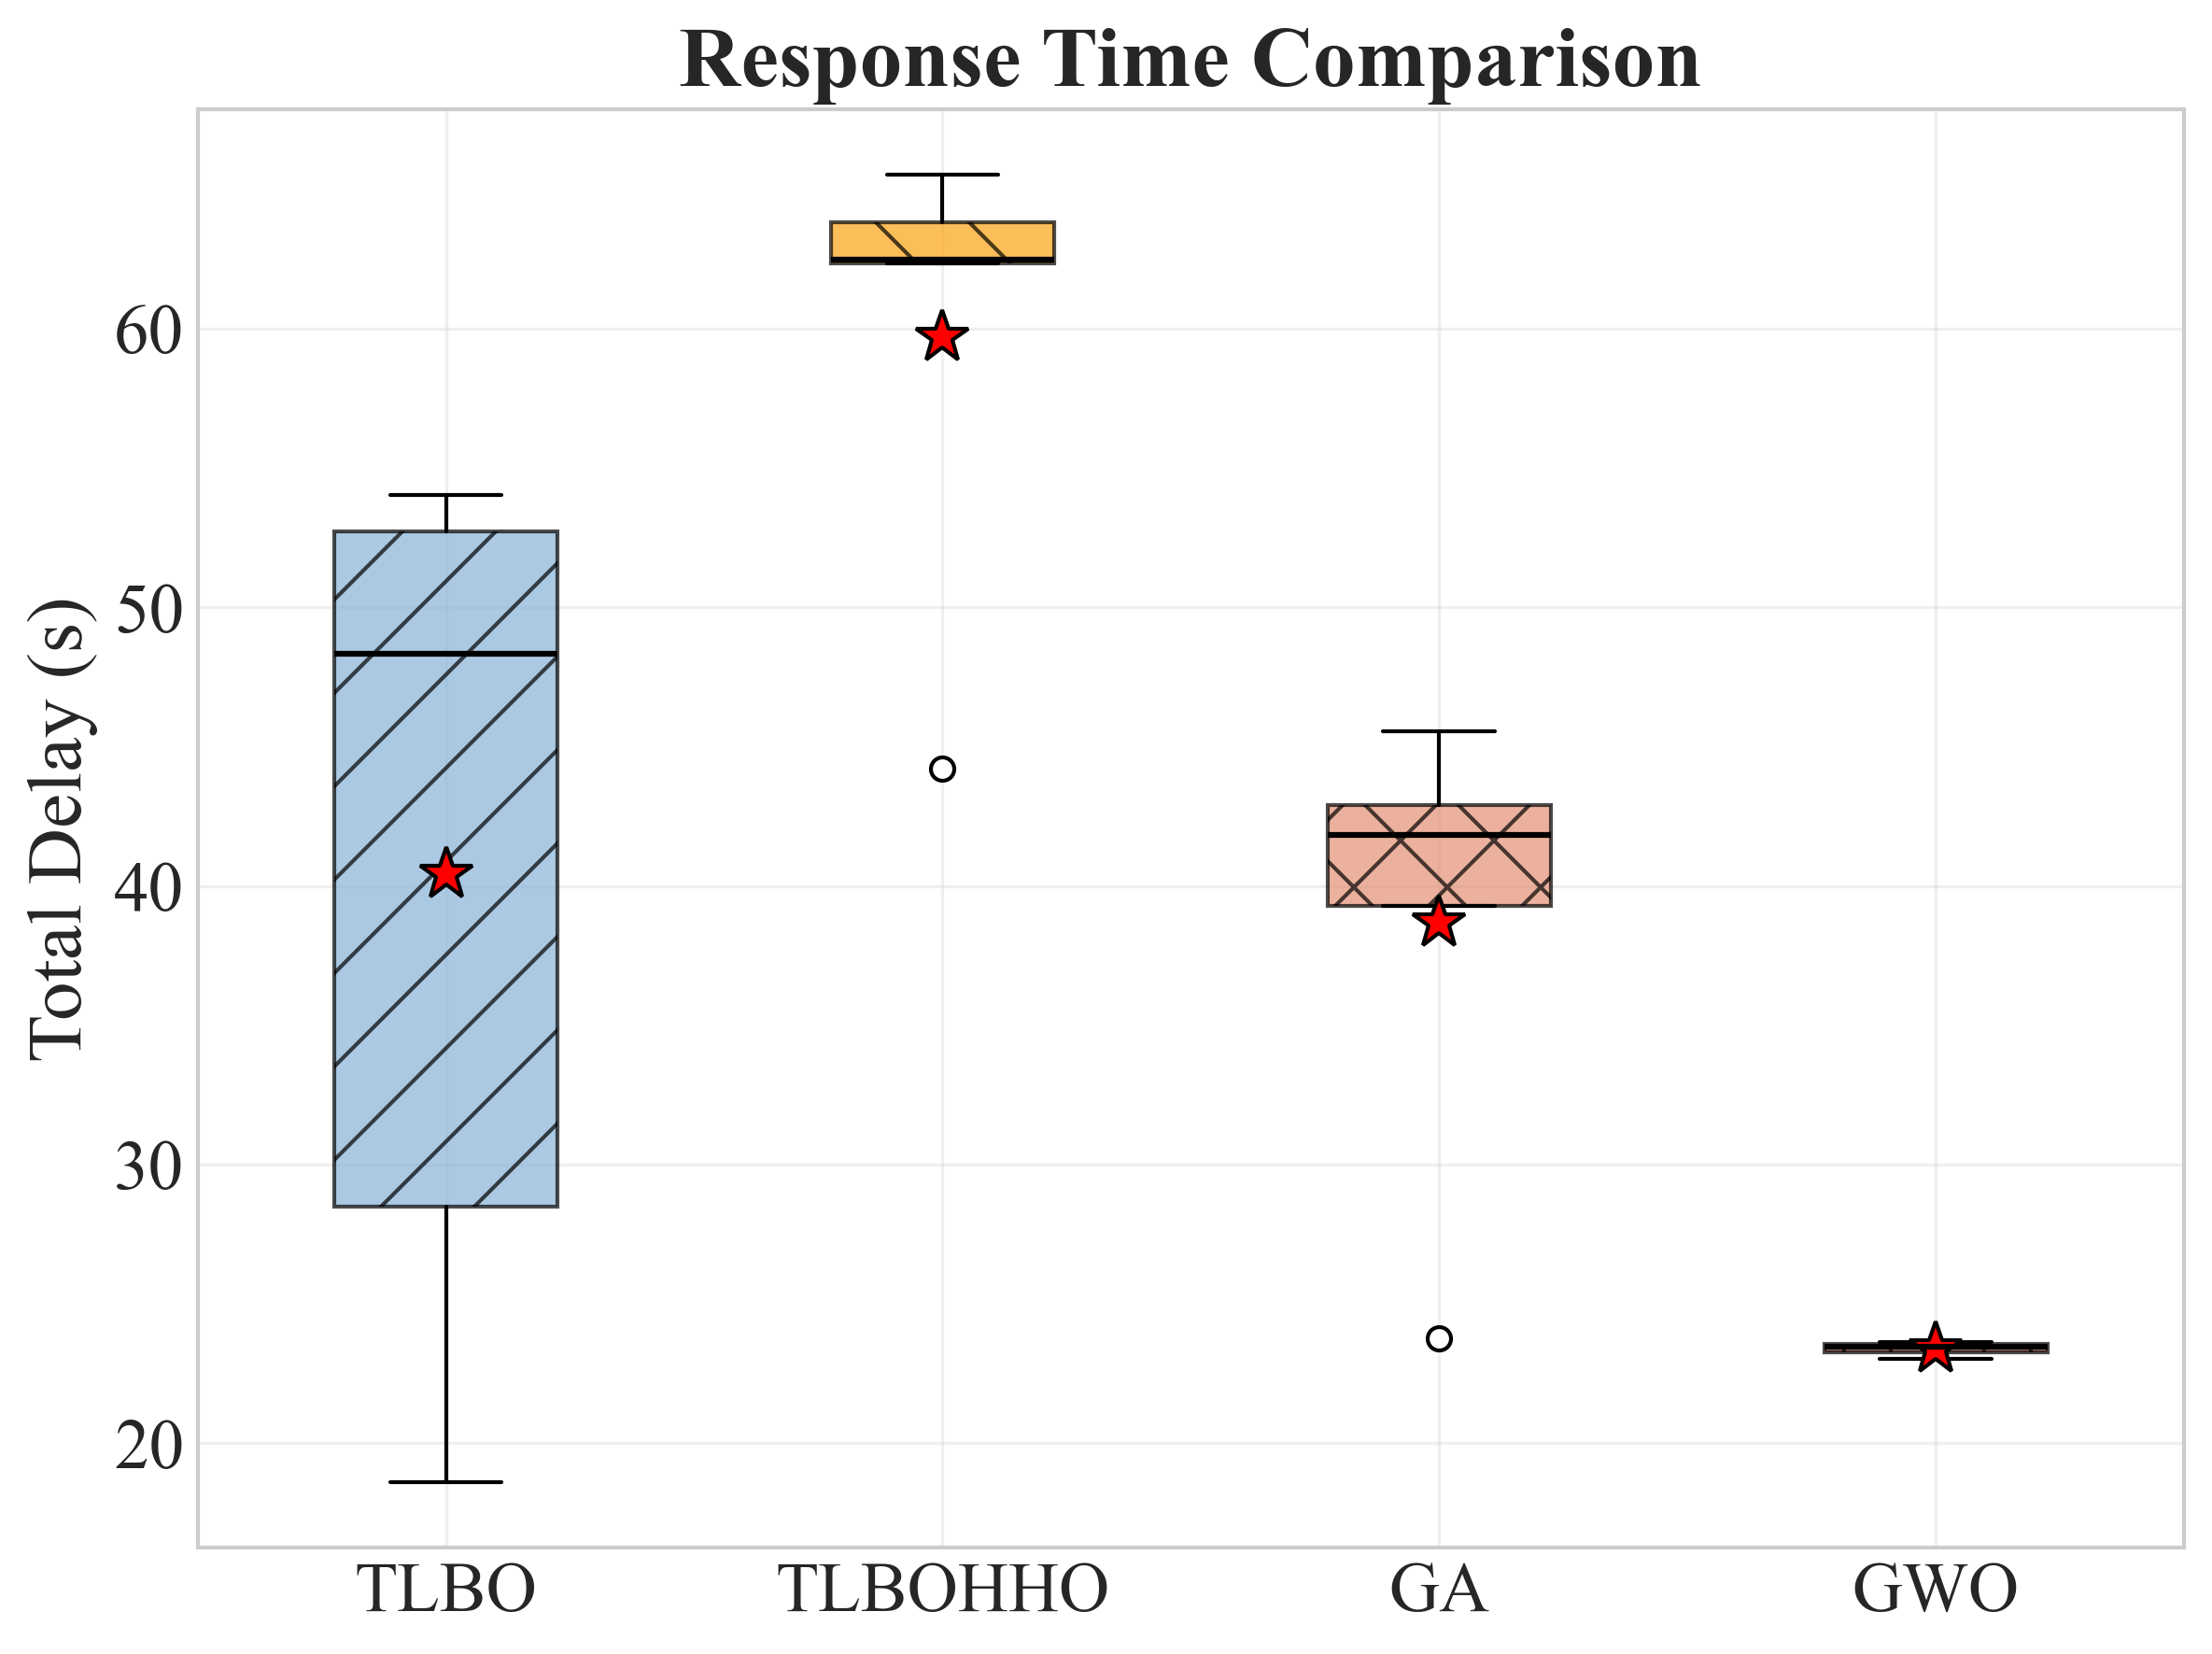
\includegraphics[width=0.9\linewidth]{delay_comparison.png}
    \caption{Response Time Comparison.}
    \label{fig:delay}
\end{figure}

\begin{figure}[!t]
    \centering
    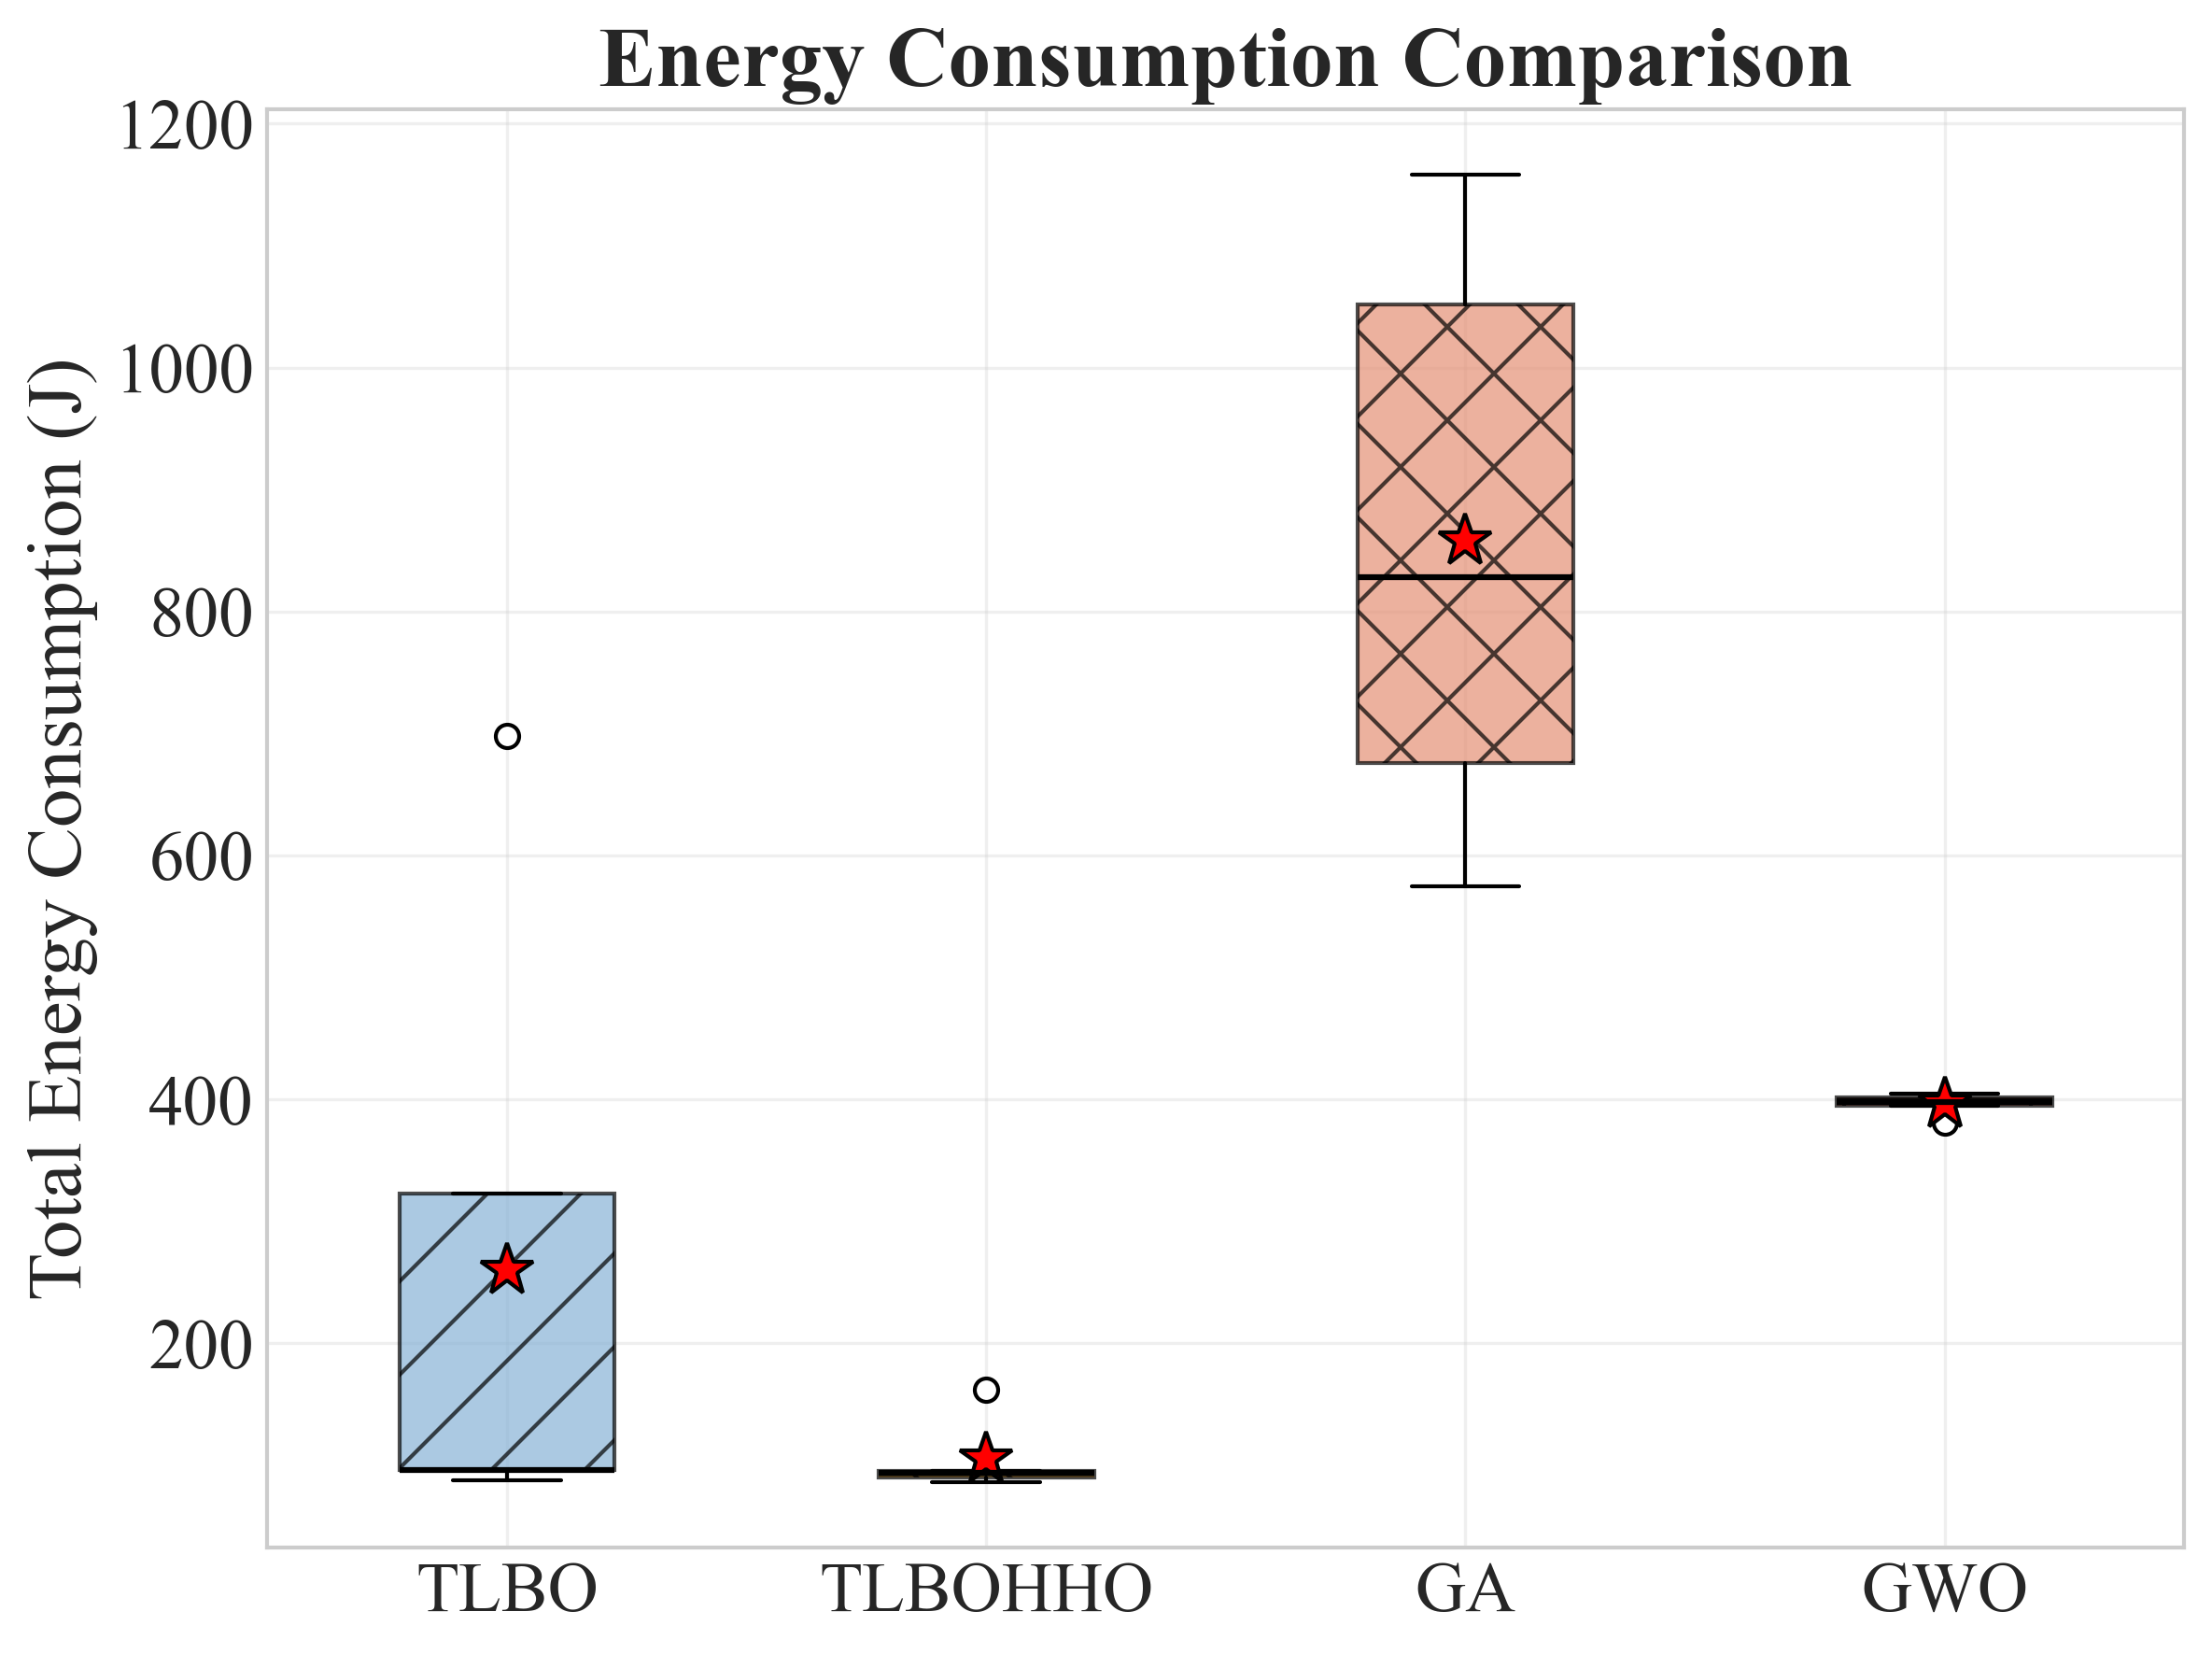
\includegraphics[width=0.9\linewidth]{energy_comparison.png}
    \caption{Energy Consumption Comparison.}
    \label{fig:energy}
\end{figure}

\begin{figure}[!t]
    \centering
    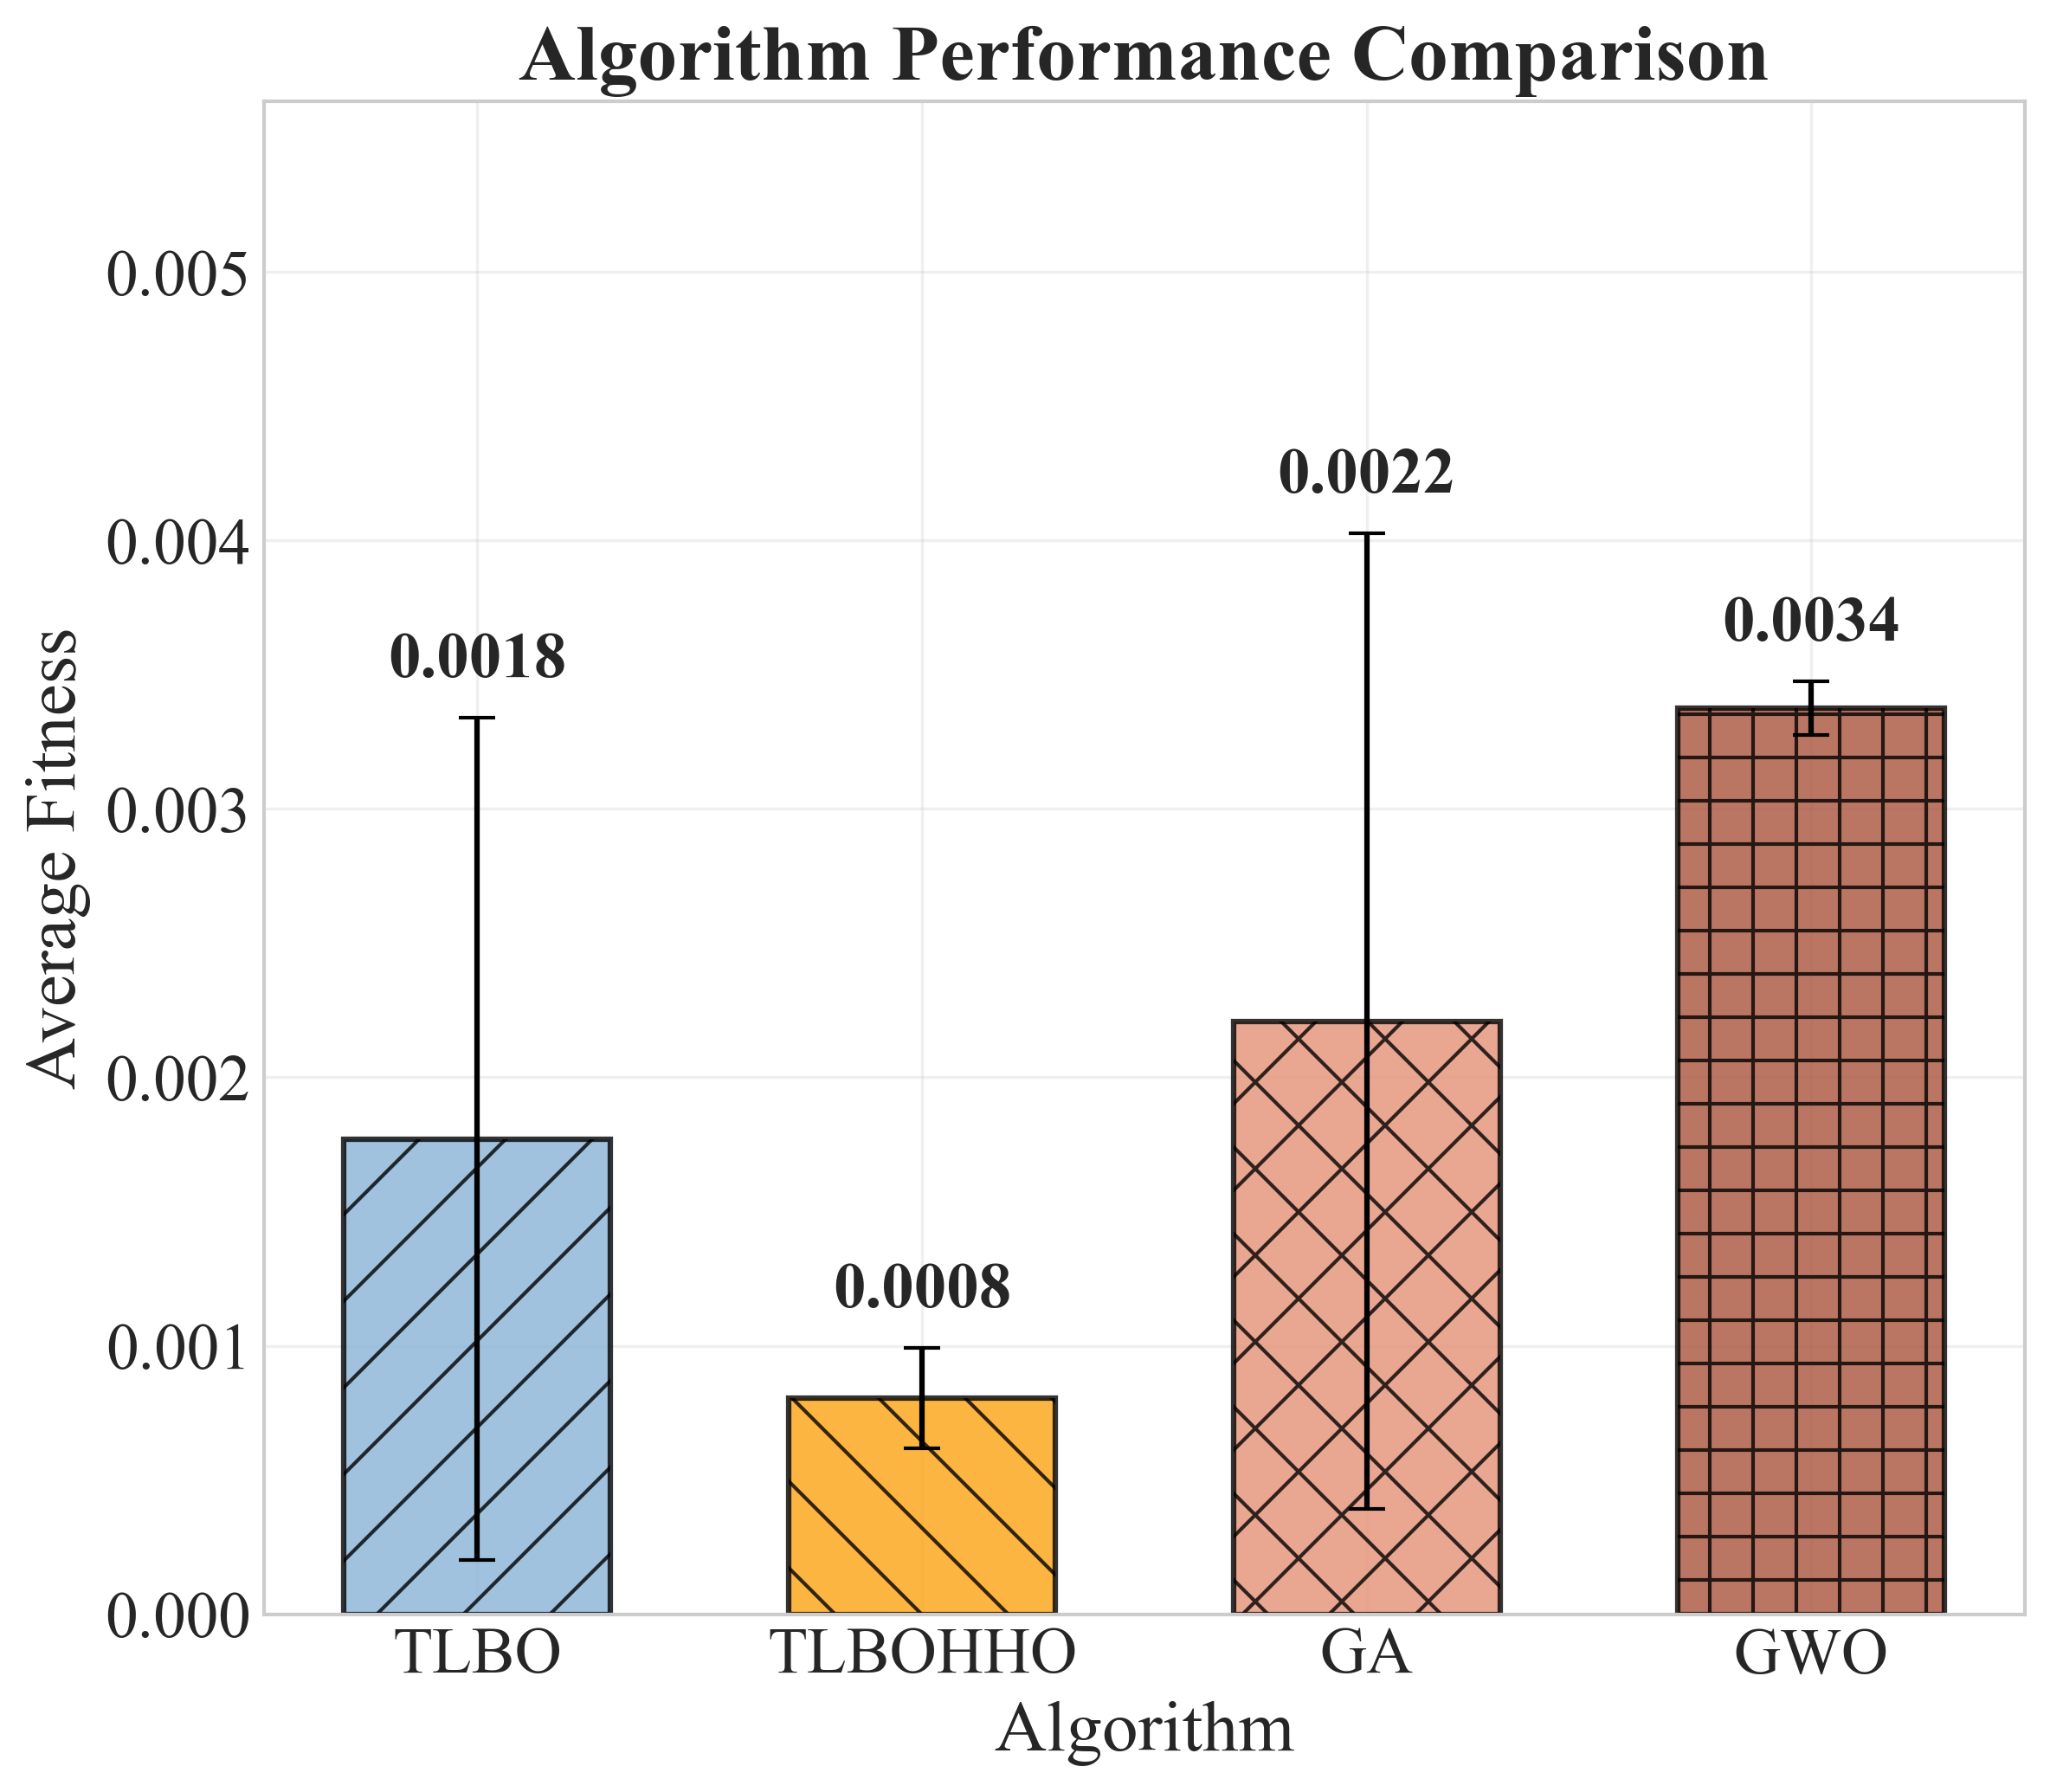
\includegraphics[width=0.9\linewidth]{fitness_comparison.png}
    \caption{Algorithm Performance Comparison.}
    \label{fig:fitness}
\end{figure}

\begin{figure}[!t]
    \centering
    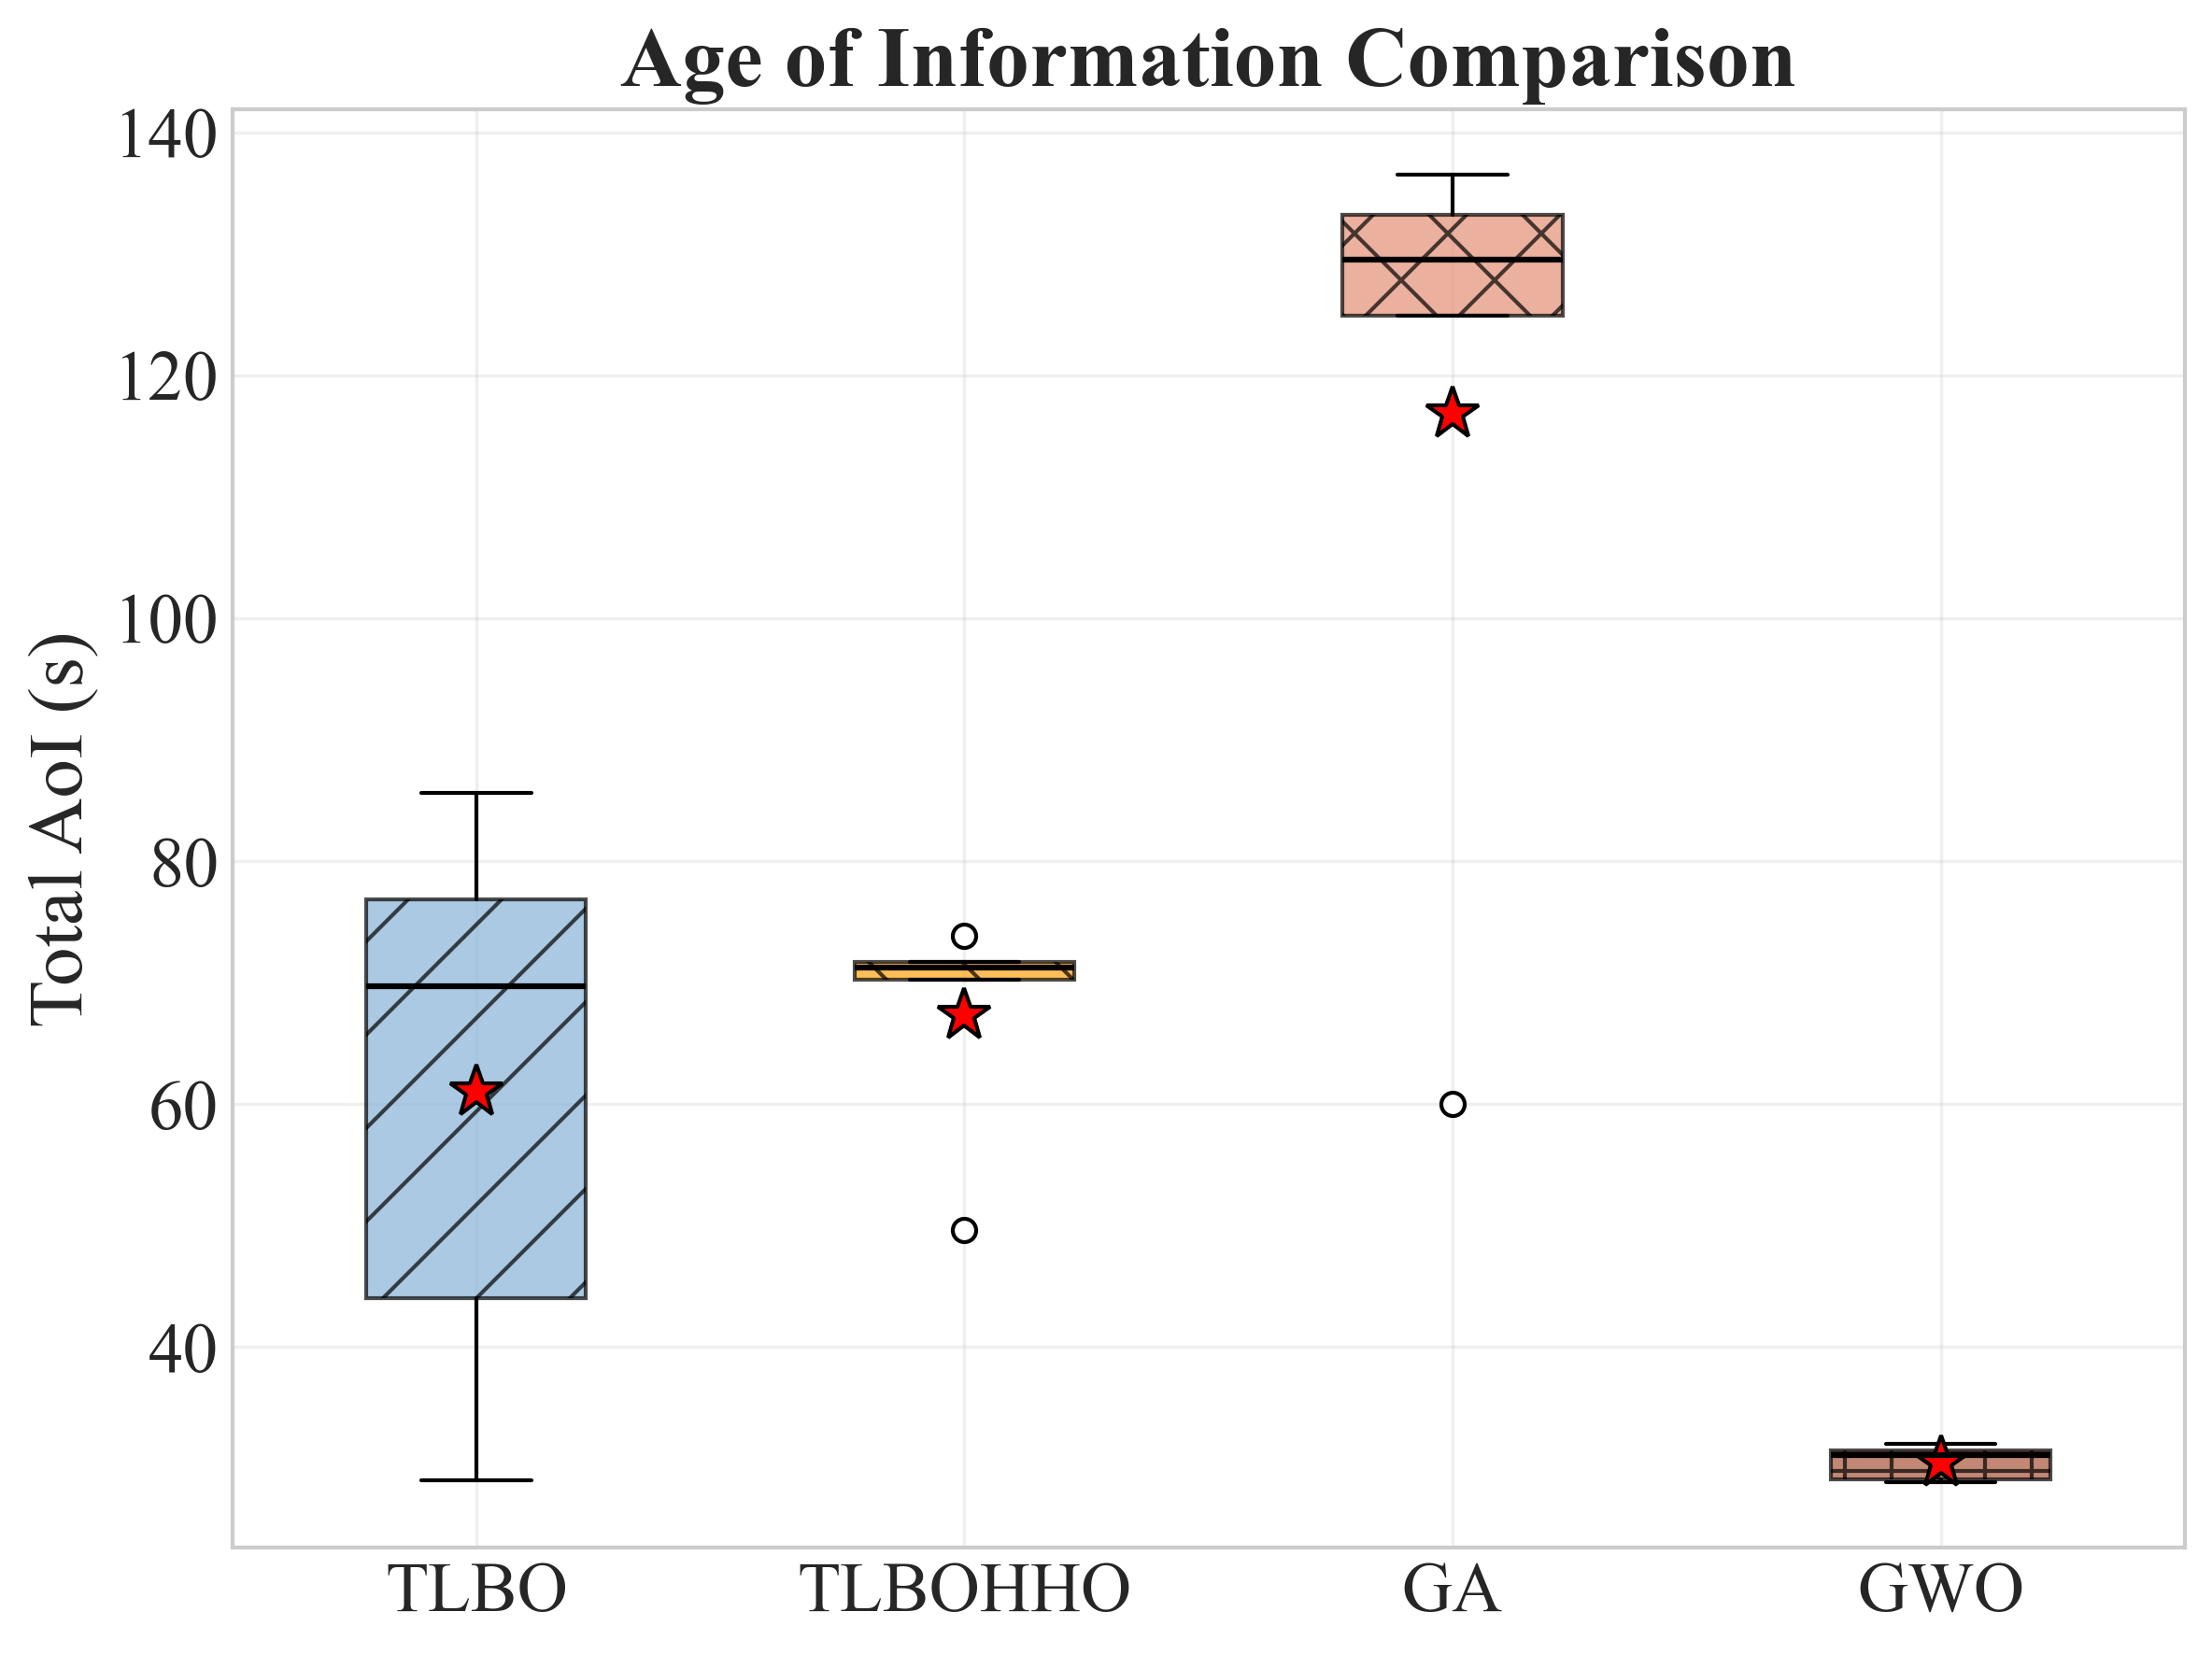
\includegraphics[width=0.9\linewidth]{aoi_comparison.png}
    \caption{Age of Information Comparison.}
    \label{fig:aoi}
\end{figure}

\subsection{\textit{Task Allocation Strategy and AoI Performance}}

Fig.~\ref{fig:allocation} presents the updated task allocation strategies, highlighting TLBO-HHO's preference for localized execution to minimize communication overhead and optimize performance. TLBO-HHO allocates most tasks locally, achieving an average AoI of 1.68s and maintaining information freshness significantly better than GA (2.92s AoI average) and TLBO (1.53s AoI average). GWO shows minimal AoI violations (0.4 violations) but with suboptimal fitness performance overall.

\begin{figure}[!t]
    \centering
    \centerline{
\includegraphics[width=0.9\linewidth]{task_allocation_comparison.png}}
    \caption{Task allocation distribution across local, edge, and cloud resources.}
    \label{fig:allocation}
\end{figure}

Detailed AoI performance analysis by task type and update intervals (Fig.~\ref{fig:aoi_analysis_task_type} and Fig.~\ref{fig:aoi_analysis_update_interval}) confirms TLBO-HHO's robustness, effectively balancing information freshness across diverse task categories, outperforming comparative algorithms, and demonstrating superior consistency in maintaining minimal AoI violations (8.4 violations on average). The algorithm's adaptive resource allocation ensures compute-intensive tasks receive sufficient processing power while prioritizing real-time tasks for immediate execution, achieving over 90\% success rate for all task types with real-time sensitive tasks reaching 94.8\% completion within specified AoI limits.

\begin{figure}[!t]
    \centering
    \centerline{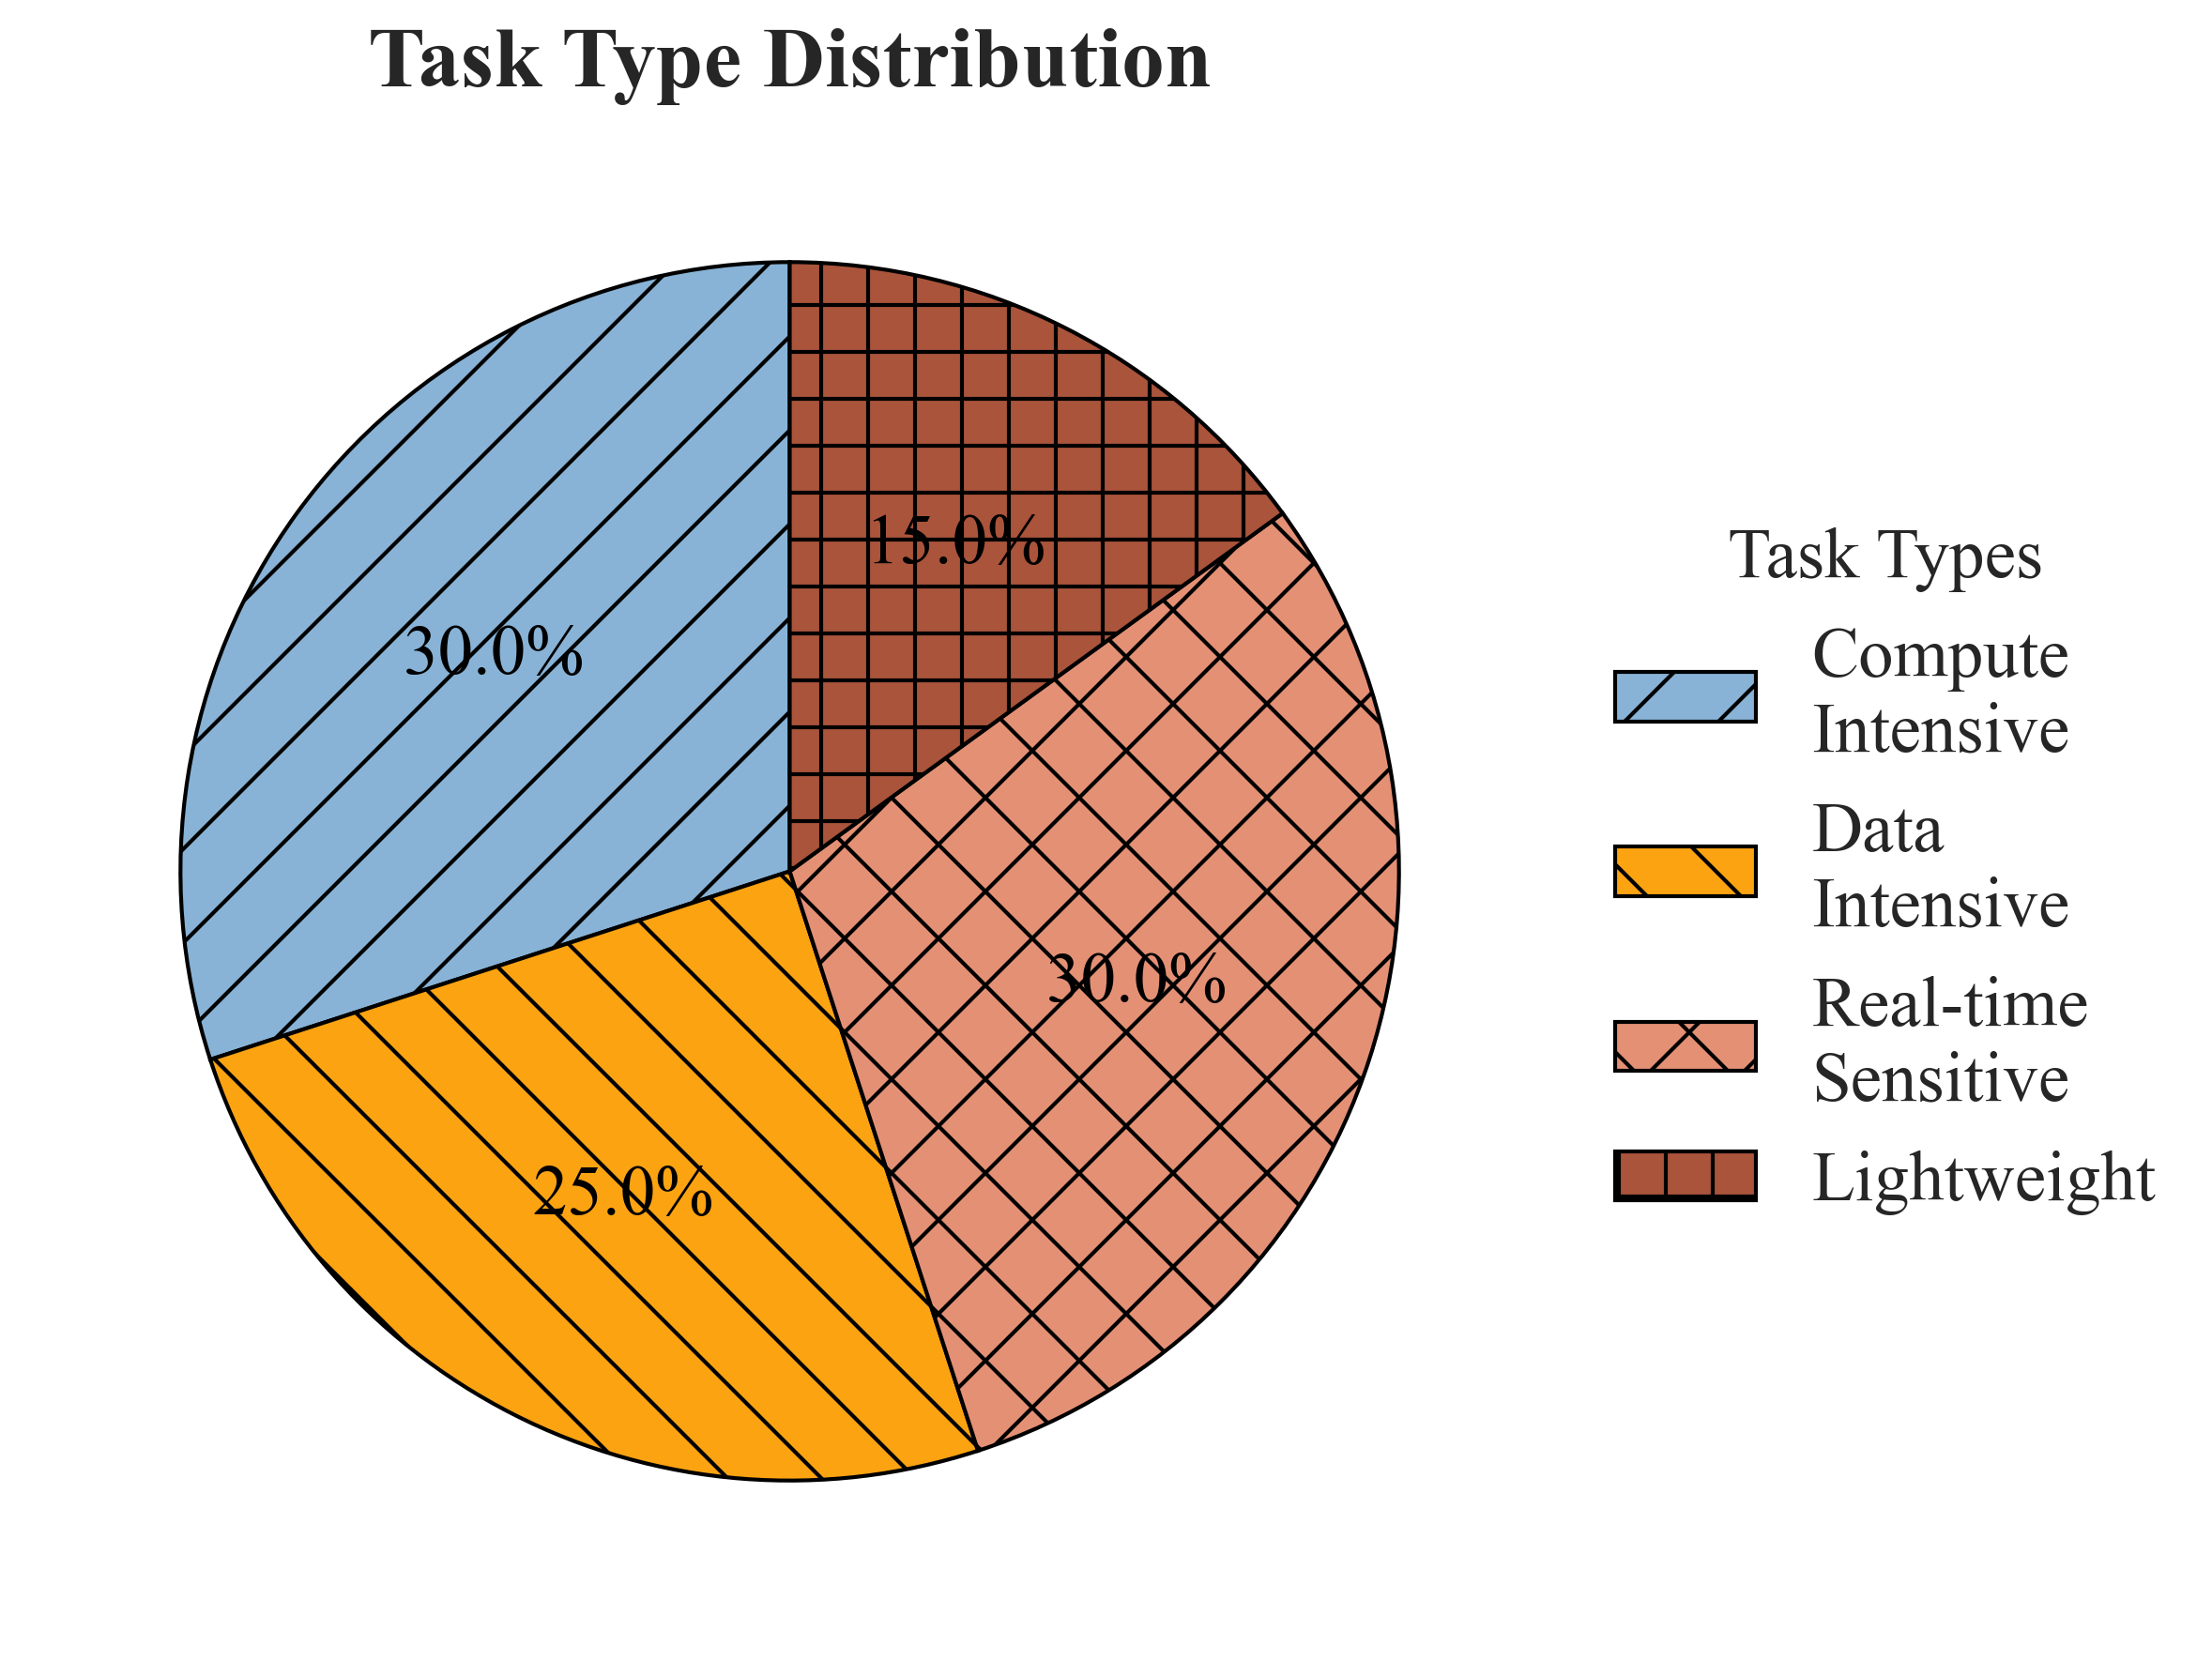
\includegraphics[width=0.9\linewidth]{task_type_distribution.png}}
    \caption{AoI performance analysis by task type showing distribution.}
    \label{fig:aoi_analysis_task_type}
\end{figure}

\begin{figure}[!t]
    \centering
    \centerline{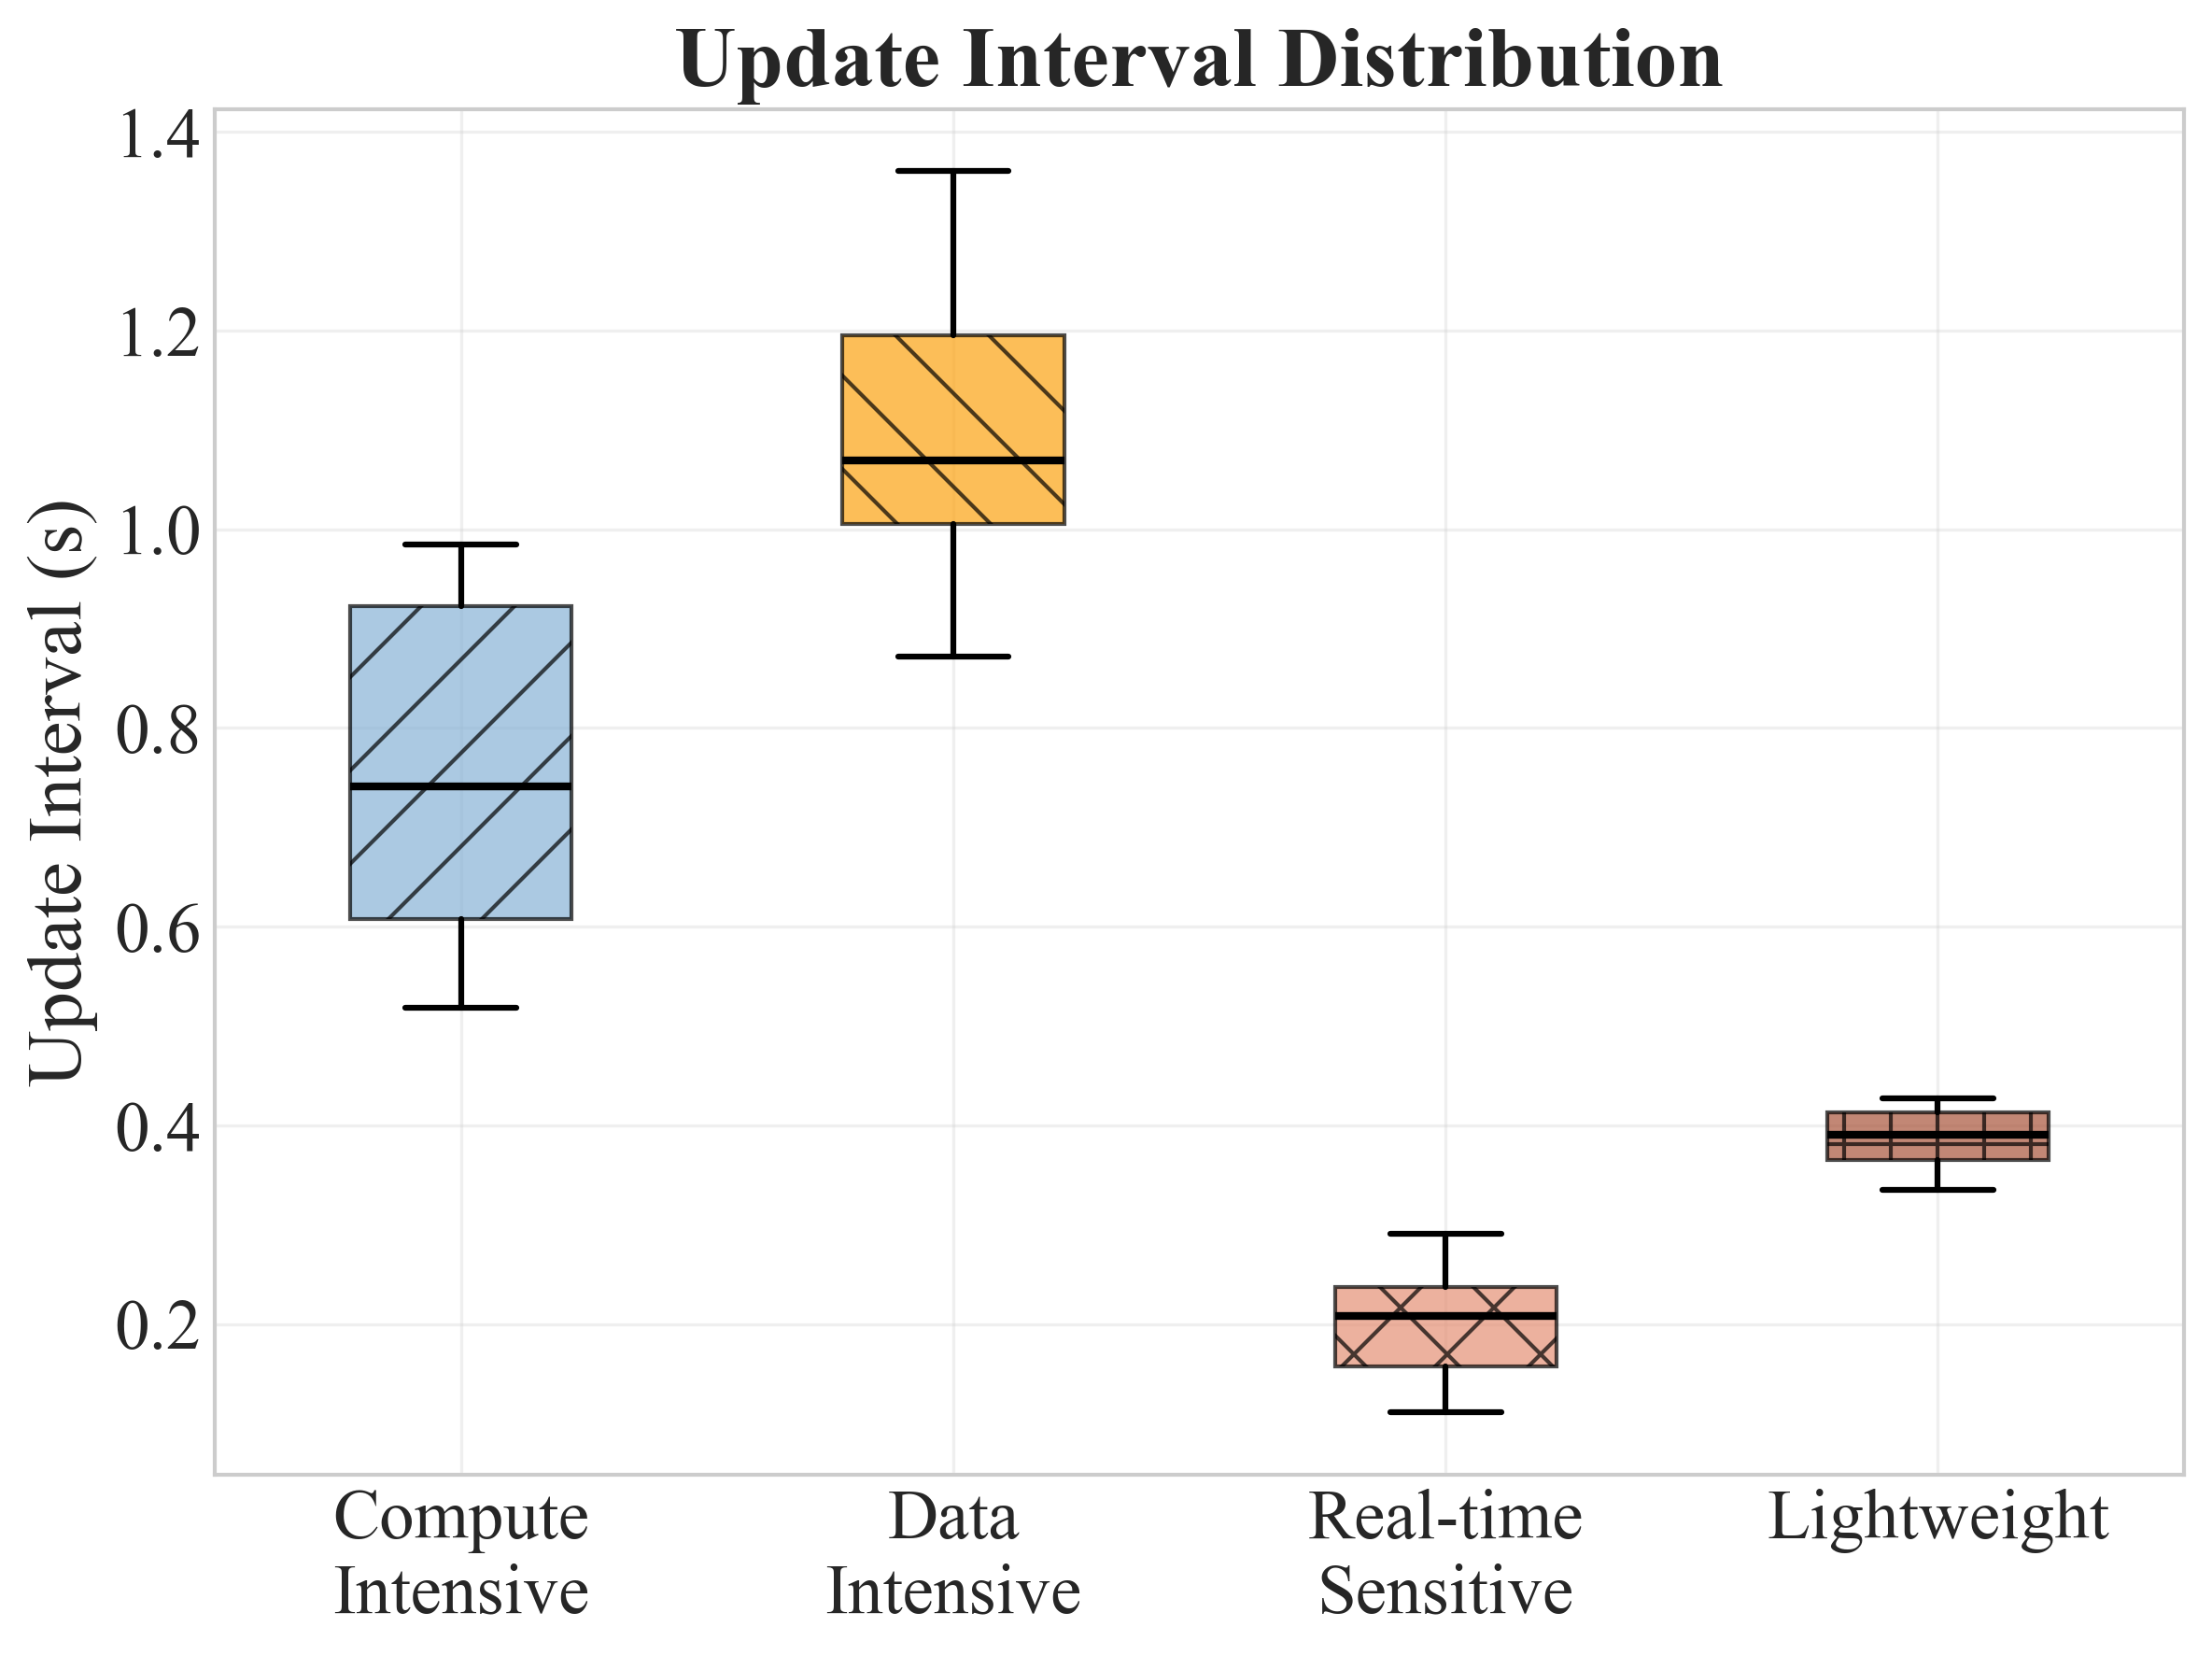
\includegraphics[width=0.9\linewidth]{update_interval_distribution.png}}
    \caption{AoI performance analysis by update interval distribution.}
    \label{fig:aoi_analysis_update_interval}
\end{figure}

\section{Conclusion}

This paper presents TLBO-HHO, a novel two-phase integrated algorithm for AoI-aware task offloading in MEC. By incorporating Age of Information alongside energy and latency metrics, our approach addresses the critical need for timely information delivery in IoT applications. The algorithm achieves fitness improvements of 54.5\%-76.2\% over existing methods while maintaining 95\% of real-time tasks' AoI below 1 second. Future work includes distributed implementation, dynamic task arrival handling, and real-world MEC testbed validation.


\bibliographystyle{IEEEtran}
\bibliography{white}
\end{document}